%!TEX program = xelatex
%!TEX encoding = UTF-8 Unicode
\documentclass{SYSUReport}

% 设置章节编号为汉字形式
\renewcommand{\thesection}{\chinese{section}}
\renewcommand{\thesubsection}{(\chinese{subsection})}
\renewcommand{\thesubsubsection}{\chinese{subsubsection}}

% 添加float包
\usepackage{float}

% 设置字体和行间距
\usepackage{fontspec}
\setmainfont{Times New Roman}
\setCJKmainfont{SimSun}
\setmonofont{Consolas}
\renewcommand{\baselinestretch}{1.5}
\linespread{1.5}

% 添加中文支持包
\usepackage{xeCJK}
\usepackage{indentfirst}
\setlength{\parindent}{2em}

% 修复页眉高度警告
\setlength{\headheight}{14.5pt}

% 添加listings包配置
\usepackage{listings}
\lstset{
    basicstyle=\ttfamily,
    breaklines=true,
    frame=single,
    numbers=none,
    showstringspaces=false,
    escapeinside={\%*}{*)},
    literate={_}{\textunderscore}1
}

% 添加超链接支持
\usepackage{hyperref}
\hypersetup{
    colorlinks=true,
    linkcolor=blue,
    filecolor=magenta,
    urlcolor=blue,
    pdftitle={图书管理系统报告},
    pdfpagemode=FullScreen,
}

% 自定义页眉样式
\usepackage{fancyhdr}
\pagestyle{fancy}
\fancyhf{} % 清除所有页眉页脚
\renewcommand{\headrulewidth}{0pt} % 移除页眉线
\fancyhead[L]{\thepage} % 左侧显示页码
\fancyhead[R]{\fontsize{9}{10}\selectfont\CJKfamily{SimSun}23336201 饶鹏程} % 右侧显示学号和姓名

% 根据个人情况修改
\lessonTitle{软件工程项目报告}
\reportTitle{基于cursor辅助的图书管理软件开发}
\stuname{饶鹏程}
\stuid{23336201}
\inst{计算机学院}
\major{计算机科学与技术}
\date{\today}

\begin{document}

% =============================================
% Part 1: 封面
% =============================================
\cover
\thispagestyle{empty} % 首页不显示页码
\clearpage

% =============================================
% Part 2: 摘要
% =============================================
%\begin{abstract}
%
%在此填写摘要内容
%
%\end{abstract}
% \thispagestyle{empty} % 摘要页不显示页码
% \clearpage


% =============================================
% Part 3: 目录页
% =============================================
% 重置页码,并使用罗马数字
\pagenumbering{Roman}
\setcounter{page}{1}
\tableofcontents
\clearpage

% =============================================
% Part 4: 正文内容
% =============================================
% 重置页码,并使用阿拉伯数字
\pagenumbering{arabic}
\setcounter{page}{1}

%%可选择这里也放一个标题
%\begin{center}
%    \title{ \Huge \textbf{{标题}}}
%\end{center}

%\vspace*{0}
\section{项目介绍}
本软件是一款基于cursor ai agent辅助开发的图书管理软件,具备添加图书、多种方式查找图书、借阅或归还图书、删除图书等基本功能。支持.txt、.pdf、.epub等多种格式的图书上传,可以添加自定义封面。本项目的github仓库地址:\url{https://github.com/seevilador/library}

\subsection{软件结构}
本软件采用Flask框架开发,采用MVC架构模式,主要包含以下几个部分:

\begin{itemize}
    \item \textbf{Model}:使用SQLAlchemy ORM框架实现,包含Book数据,存储图书的所有属性和关系,包括:
    \begin{itemize}
        \item 基本属性:标题、作者、ISBN、出版日期、分类、描述
        \item 文件信息:电子书文件路径、封面图片路径
        \item 借阅信息:借出状态、借阅者、借阅日期、归还日期
        \item 时间戳:创建时间、更新时间
    \end{itemize}
    
    \item \textbf{View}:使用HTML实现,位于templates目录下,包括:
    \begin{itemize}
        \item index.html:首页,显示图书列表和搜索功能
        \item 其他页面
    \end{itemize}
    
    \item \textbf{Controller}:在app.py中实现,包含主要功能:
    \begin{itemize}
        \item 图书管理和编辑:添加、编辑、删除图书
        \item 借阅管理:借出、归还图书
        \item 文件处理:上传、下载电子书和封面图片
        \item 搜索图书:支持按标题、作者、ISBN、分类搜索
    \end{itemize}
    
    \item \textbf{静态资源}:位于static目录,包括:
    \begin{itemize}
        \item CSS文件
        \item JS脚本
        \item 图片(封面)
    \end{itemize}
    
    \item \textbf{数据存储}:
    \begin{itemize}
        \item 数据库:使用SQL存储图书信息和属性
        \item 文件:存储电子书文件和封面图片
    \end{itemize}
\end{itemize}

软件的文件结构如下:
\begin{verbatim}
library/
├── app.py              # 主程序
├── database.py         # 数据库
├── requirements.txt    # 依赖包列表
├── templates/          # HTML
├── static/            # 静态资源
│   ├── css/          # 样式
│   ├── js/           # JS文件
│   └── covers/       # 封面图片
├── uploads/           # 上传的电子书文件
└── .specstory/       # 开发历史记录
\end{verbatim}

\vspace*{1cm}
\section{软件开发}
\subsection{开发流程概述}
本软件是基于ai agent的代码实现功能,由开发者任务驱动开发的软件。抽象的开发过程为开发者分析软件功能,得出开发需求并提供给ai编程实现,开发者再对代码进行测试并提出改进或新需求的交替实现。

\begin{figure}[H]
    \centering
    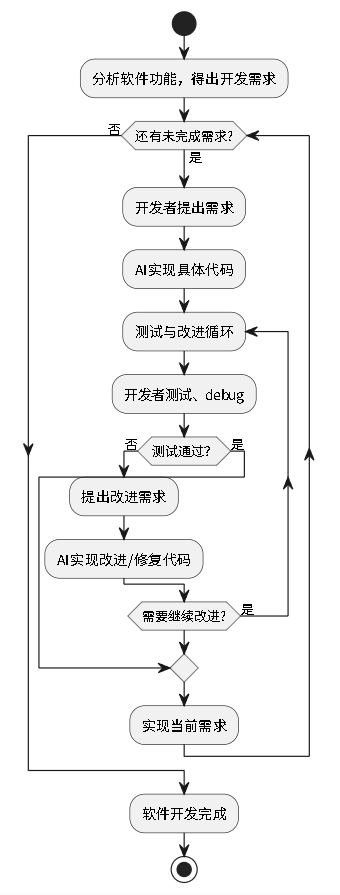
\includegraphics[width=0.3\textwidth]{figures/流程.png}
    \caption{软件开发流程图}
    \label{fig:flow}
\end{figure}

与ai agent对话辅助开发的完整历史存放在\textbackslash .specstory\textbackslash history 中。


\section{功能实现}

\subsection{添加图书功能}
添加图书功能主要通过以下代码实现:

\begin{lstlisting}[language=Python]
@app.route('/add', methods=['POST'])
def add_book():
    try:
        # 获取表单数据
        title = request.form.get('title')
        author = request.form.get('author')
        isbn = request.form.get('isbn')
        publish_date_str = request.form.get('publish_date')
        category = request.form.get('category')
        description = request.form.get('description')
        
        # 处理图书文件
        file_path = None
        if 'file' in request.files:
            file = request.files['file']
            if file.filename != '' and allowed_file(file.filename):
                filename = secure_filename(file.filename)
                file_path = os.path.join(app.config['UPLOAD_FOLDER'], filename)
                file.save(file_path)
        
        # 处理封面图片
        cover_path = None
        if 'cover' in request.files:
            cover = request.files['cover']
            if cover.filename != '' and allowed_image(cover.filename):
                cover_filename = secure_filename(cover.filename)
                cover_path = f"covers/{cover_filename}"
                full_cover_path = os.path.join(app.config['COVER_FOLDER'], cover_filename)
                cover.save(full_cover_path)
        
        # 创建图书对象并保存到数据库
        if title and author:
            book = Book(
                title=title,
                author=author,
                isbn=isbn,
                publish_date=datetime.strptime(publish_date_str, '%Y-%m-%d').date() if publish_date_str else None,
                category=category,
                description=description,
                file_path=file_path,
                cover_path=cover_path
            )
            db.session.add(book)
            db.session.commit()
            flash('图书添加成功!')
    except Exception as e:
        logger.error(f"添加图书时出错: {str(e)}")
        flash('添加图书时出错,请查看日志')
    
    return redirect(url_for('index'))
\end{lstlisting}

该功能的主要实现步骤包括:

\begin{enumerate}
    \item \textbf{接收表单数据}:
    \begin{lstlisting}[language=Python]
    title = request.form.get('title')
    author = request.form.get('author')
    isbn = request.form.get('isbn')
    \end{lstlisting}
    \text{通过Flask的request对象获取表单提交的图书基本信息,包括标题、作者、ISBN等字段。}
    
    \item \textbf{处理文件上传}:
    \begin{lstlisting}[language=Python]
    if 'file' in request.files:
        file = request.files['file']
        if file.filename != '' and allowed_file(file.filename):
            filename = secure_filename(file.filename)
            file_path = os.path.join(app.config['UPLOAD_FOLDER'], filename)
            file.save(file_path)
    \end{lstlisting}
    \text{使用Flask的文件上传功能处理电子书文件,通过secure\_filename确保文件名安全,并将文件保存到指定目录。}
    
    \item \textbf{处理封面图片}:
    \begin{lstlisting}[language=Python]
    if 'cover' in request.files:
        cover = request.files['cover']
        if cover.filename != '' and allowed_image(cover.filename):
            cover_filename = secure_filename(cover.filename)
            cover_path = f"covers/{cover_filename}"
            full_cover_path = os.path.join(app.config['COVER_FOLDER'], cover_filename)
            cover.save(full_cover_path)
    \end{lstlisting}
    \text{类似地处理封面图片上传,使用相对路径存储图片引用。}
    
    \item \textbf{数据验证和保存}:
    \begin{lstlisting}[language=Python]
    if title and author:
        book = Book(
            title=title,
            author=author,
            isbn=isbn,
            publish_date=datetime.strptime(publish_date_str, '%Y-%m-%d').date() if publish_date_str else None,
            category=category,
            description=description,
            file_path=file_path,
            cover_path=cover_path
        )
        db.session.add(book)
        db.session.commit()
    \end{lstlisting}
    \text{验证必填字段(标题和作者),创建Book对象并保存到数据库。}
    
    \item \textbf{错误处理}:
    \begin{lstlisting}[language=Python]
    try:
        # ... 主要代码 ...
    except Exception as e:
        logger.error(f"添加图书时出错: {str(e)}")
        flash('添加图书时出错,请查看日志')
    \end{lstlisting}
    \text{使用try-except捕获可能的异常,记录错误日志并显示用户友好的提示信息。}
\end{enumerate}

\subsection{借阅图书功能}
借阅图书功能通过以下代码实现:

\begin{lstlisting}[language=Python]
@app.route('/borrow_book/<int:id>')
def borrow_book(id):
    try:
        book = Book.query.get_or_404(id)
        
        # 检查图书是否已被借出
        if book.is_borrowed:
            flash('该图书已被借出!')
            return redirect(url_for('index'))
        
        # 更新借阅信息
        book.is_borrowed = True
        book.borrower = request.args.get('borrower', '未知借阅者')
        book.borrow_date = datetime.utcnow()
        book.return_date = datetime.utcnow() + timedelta(days=30)  # 默认借阅30天
        
        db.session.commit()
        flash('借阅成功!')
    except Exception as e:
        logger.error(f"借阅图书时出错: {str(e)}")
        flash('借阅失败,请重试!')
    
    return redirect(url_for('index'))
\end{lstlisting}

借阅功能的主要实现步骤:

\begin{enumerate}
    \item \textbf{获取图书信息}:
    \begin{lstlisting}[language=Python]
    book = Book.query.get_or_404(id)
    \end{lstlisting}
    通过图书ID查询数据库,如果图书不存在则返回404错误。
    
    \item \textbf{状态检查}:
    \begin{lstlisting}[language=Python]
    if book.is_borrowed:
        flash('该图书已被借出!')
        return redirect(url_for('index'))
    \end{lstlisting}
    检查图书是否已被借出,如果已借出则显示提示信息并返回首页。
    
    \item \textbf{更新借阅信息}:
    \begin{lstlisting}[language=Python]
    book.is_borrowed = True
    book.borrower = request.args.get('borrower', '未知借阅者')
    book.borrow_date = datetime.utcnow()
    book.return_date = datetime.utcnow() + timedelta(days=30)
    \end{lstlisting}
    设置借阅状态、借阅者信息、借阅日期和预计归还日期(默认30天)。
    
    \item \textbf{保存更改}:
    \begin{lstlisting}[language=Python]
    db.session.commit()
    \end{lstlisting}
    将更改提交到数据库。
\end{enumerate}

\subsection{删除图书功能}
删除图书功能通过以下代码实现:

\begin{lstlisting}[language=Python]
@app.route('/delete_book/<int:id>')
def delete_book(id):
    try:
        book = Book.query.get_or_404(id)
        
        # 检查图书是否已借出
        if book.is_borrowed:
            flash('该图书已被借出,无法删除!请先归还图书。')
            return redirect(url_for('index'))
        
        # 删除相关文件
        if book.file_path and os.path.exists(book.file_path):
            os.remove(book.file_path)
        
        if book.cover_path:
            cover_path = os.path.join(app.config['COVER_FOLDER'], os.path.basename(book.cover_path))
            if os.path.exists(cover_path):
                os.remove(cover_path)
        
        # 从数据库中删除记录
        db.session.delete(book)
        db.session.commit()
        flash('图书删除成功!')
    except Exception as e:
        logger.error(f"删除图书时出错: {str(e)}")
        flash('删除失败,请重试!')
    
    return redirect(url_for('index'))
\end{lstlisting}

删除功能的主要实现步骤:

\begin{enumerate}
    \item \textbf{安全检查}:
    \begin{lstlisting}[language=Python]
    if book.is_borrowed:
        flash('该图书已被借出,无法删除!请先归还图书。')
        return redirect(url_for('index'))
    \end{lstlisting}
    确保图书未被借出才能进行删除操作。
    
    \item \textbf{文件清理}:
    \begin{lstlisting}[language=Python]
    if book.file_path and os.path.exists(book.file_path):
        os.remove(book.file_path)
    
    if book.cover_path:
        cover_path = os.path.join(app.config['COVER_FOLDER'], os.path.basename(book.cover_path))
        if os.path.exists(cover_path):
            os.remove(cover_path)
    \end{lstlisting}
    删除相关的电子书文件和封面图片。
    
    \item \textbf{数据库操作}:
    \begin{lstlisting}[language=Python]
    db.session.delete(book)
    db.session.commit()
    \end{lstlisting}
    从数据库中删除图书记录。
\end{enumerate}

\section{效果展示}
使用编译形成的app.exe或者执行命令"python app.py"运行软件,然后在浏览器中访问:\url{http://localhost:5000}进入软件的webui界面。

\begin{figure}[H]
    \centering
    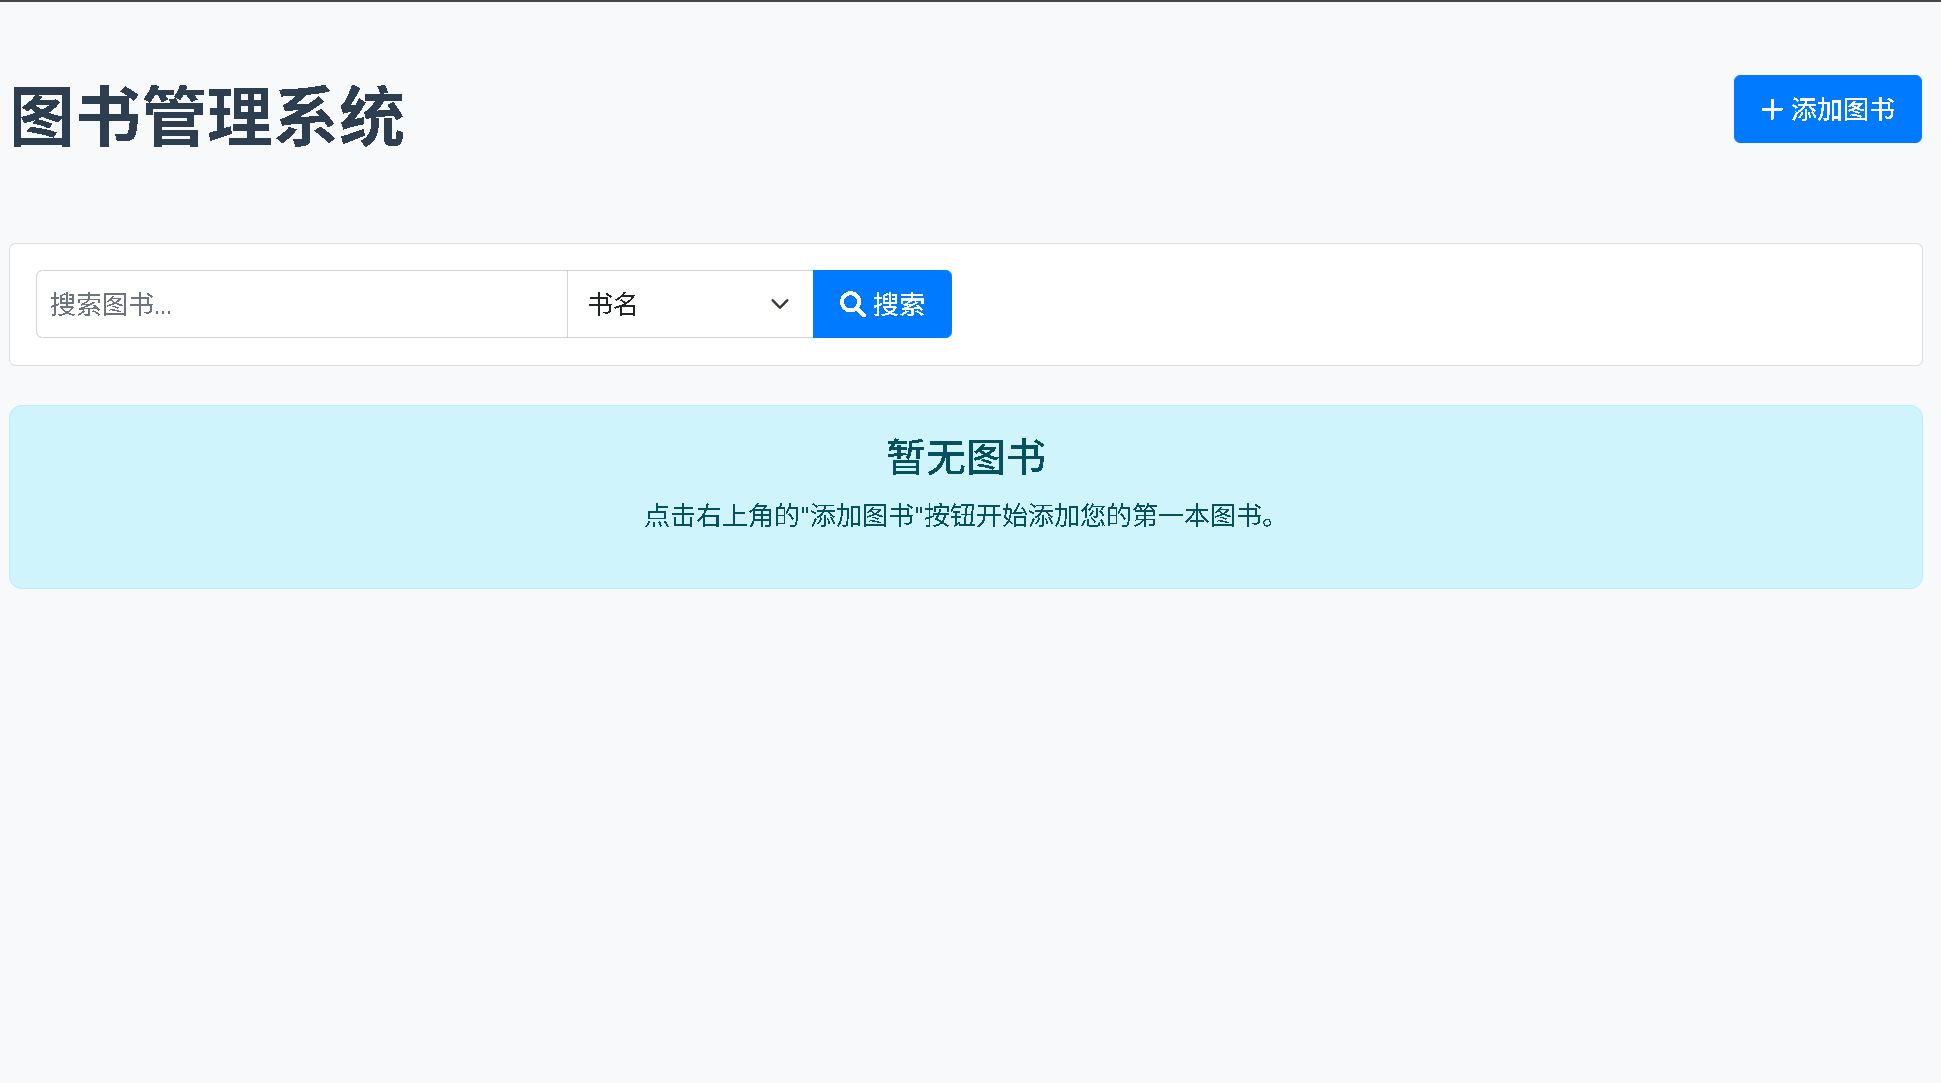
\includegraphics[width=0.9\textwidth]{figures/start_menu.png}
    \caption{起始页面}
    \label{fig:flow}
\end{figure}

单击右上角的"添加图书",即可添加图书。如果不配置封面则使用存放在\textbackslash cover中的默认封面。
\begin{figure}[H]
    \centering
    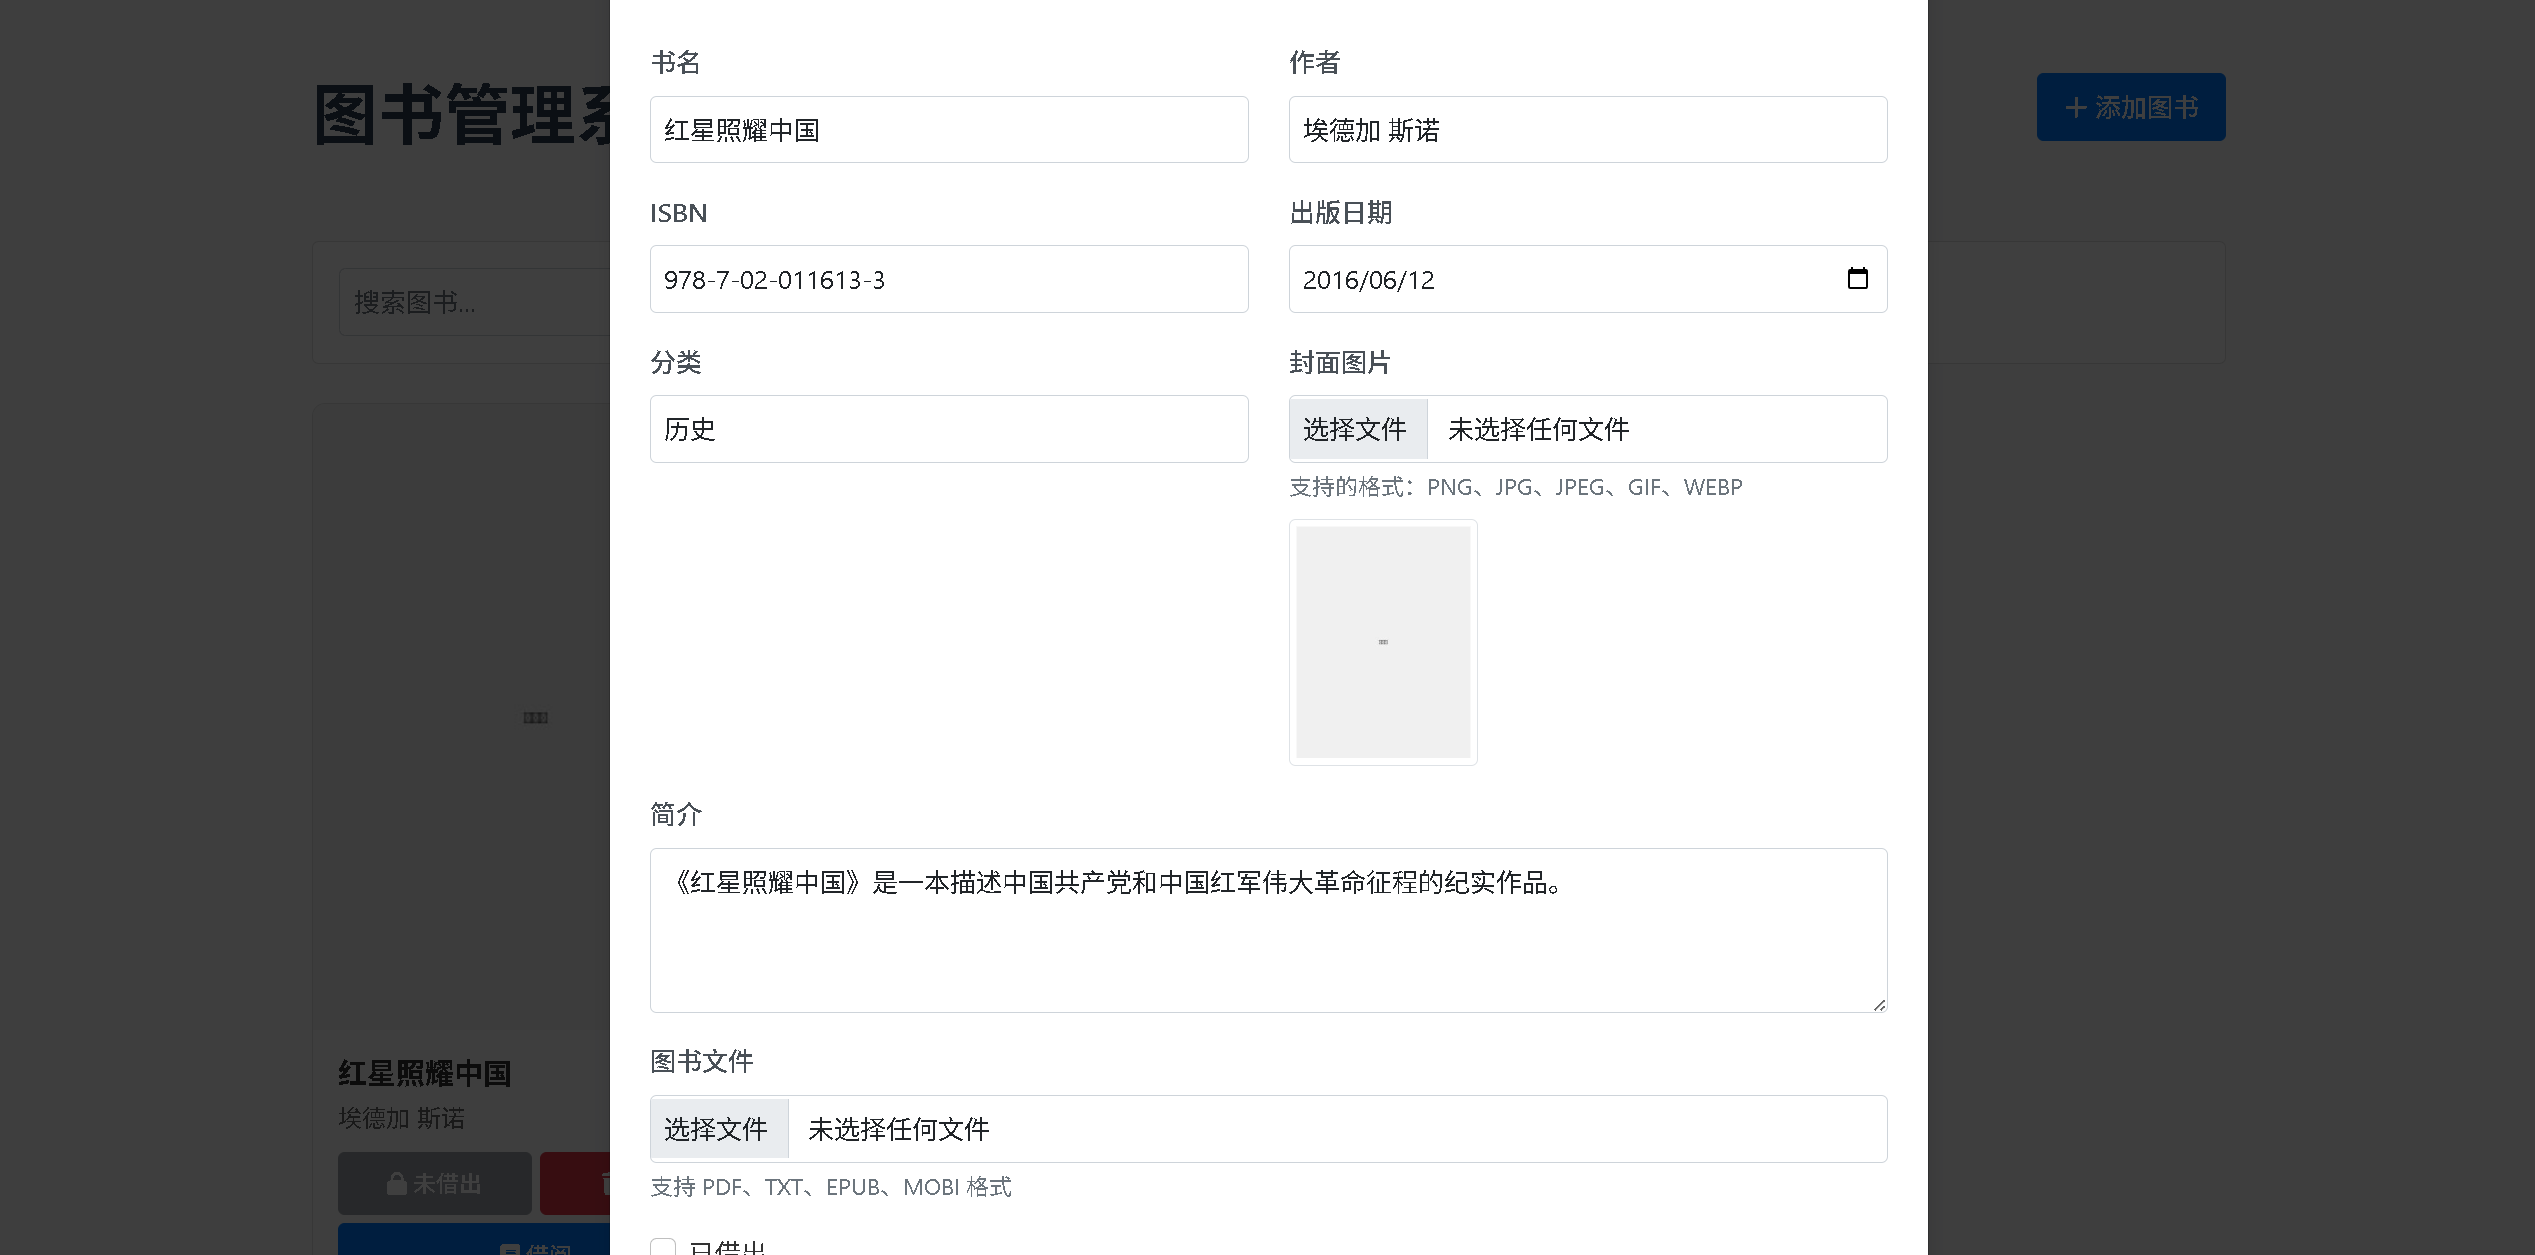
\includegraphics[width=0.9\textwidth]{figures/add_book.png}
    \caption{添加图书}
    \label{fig:flow}
\end{figure}

\begin{figure}[H]
    \centering
    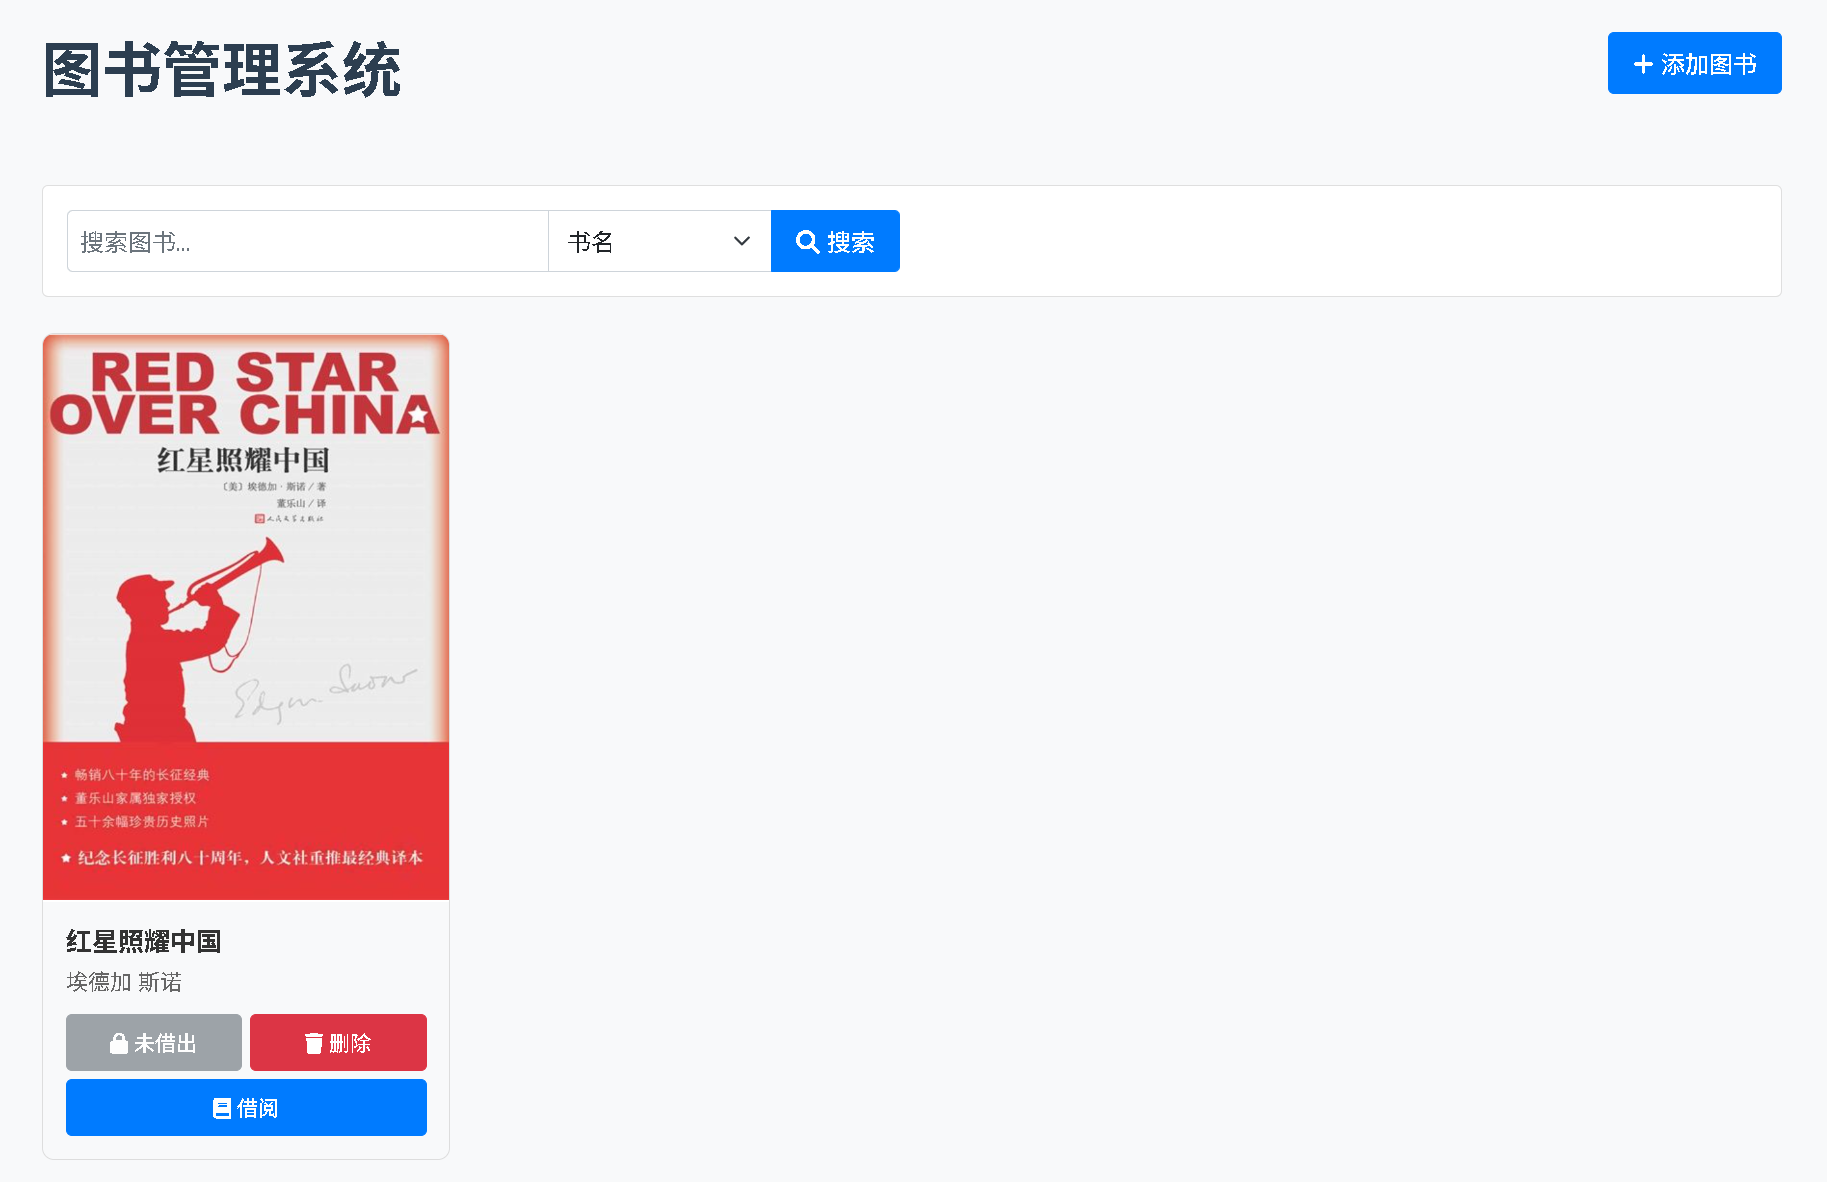
\includegraphics[width=0.9\textwidth]{figures/add_cpt.png}
    \caption{添加图书后效果}
    \label{fig:flow}
\end{figure}
添加图书后,按照属性搜索图书

\begin{figure}[H]
    \centering
    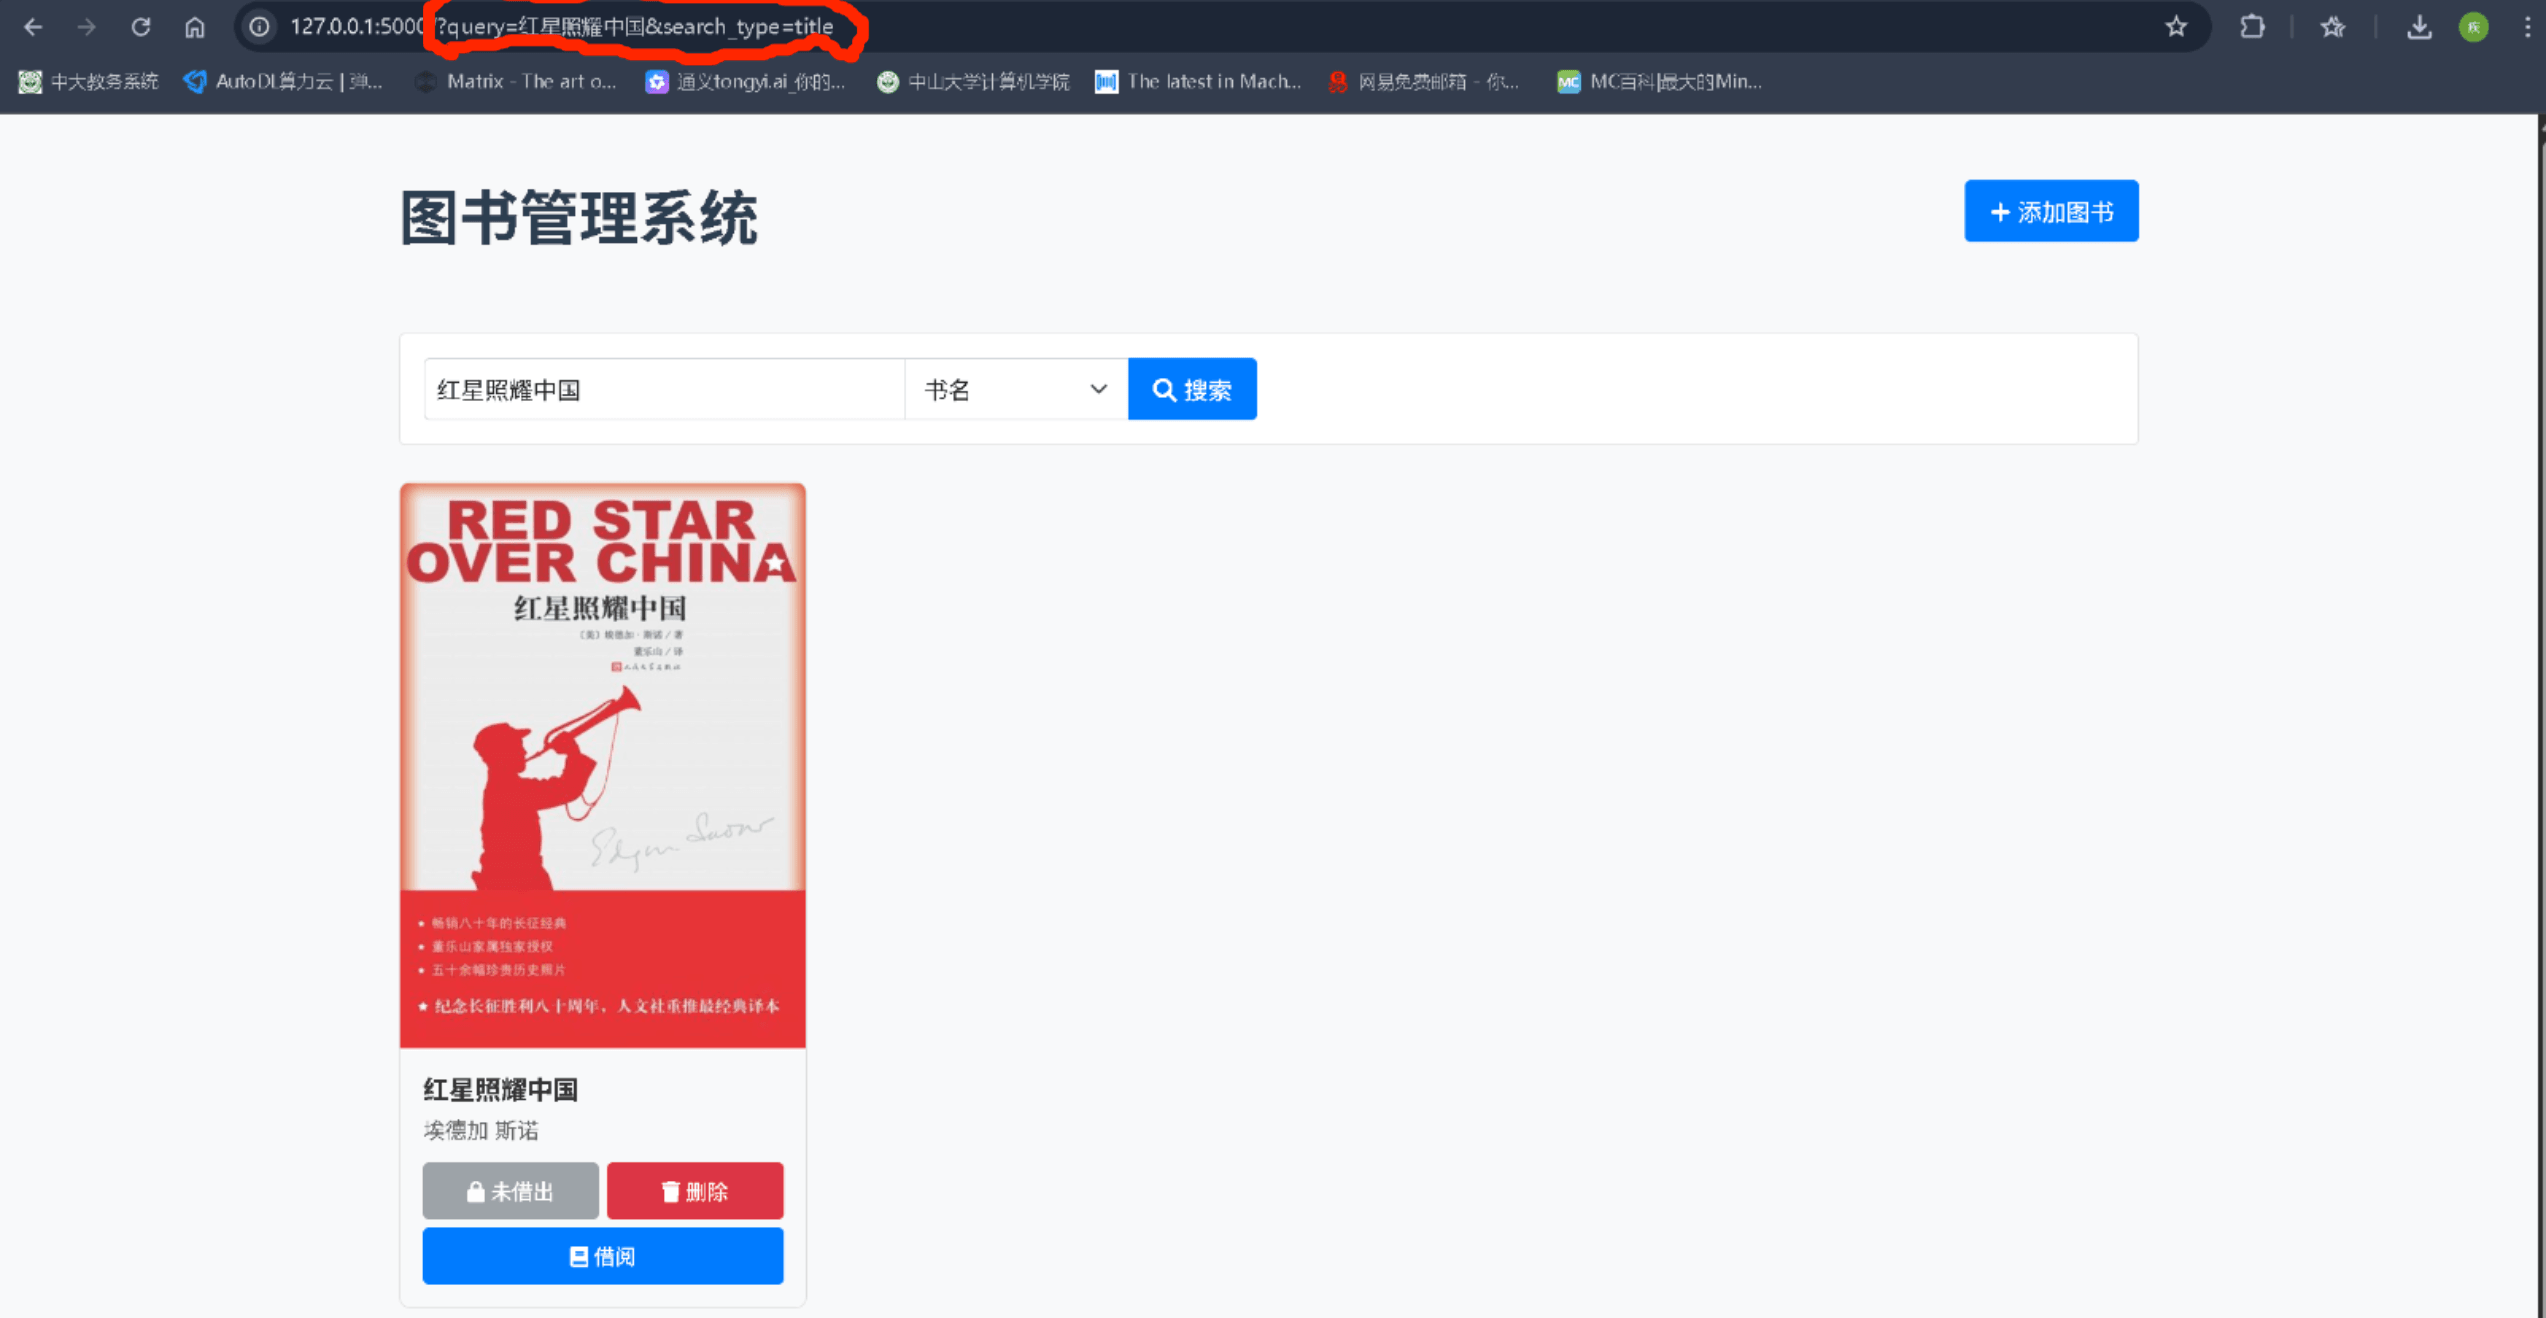
\includegraphics[width=0.9\textwidth]{figures/search_name.png}
    \caption{按照书名查找图书}
    \label{fig:flow}
\end{figure}

单击图书左下角的"借阅"或"归还",实现借阅或者归还图书。当借阅图书时,可以使用"下载"功能模拟借书。

\begin{figure}[H]
    \centering
    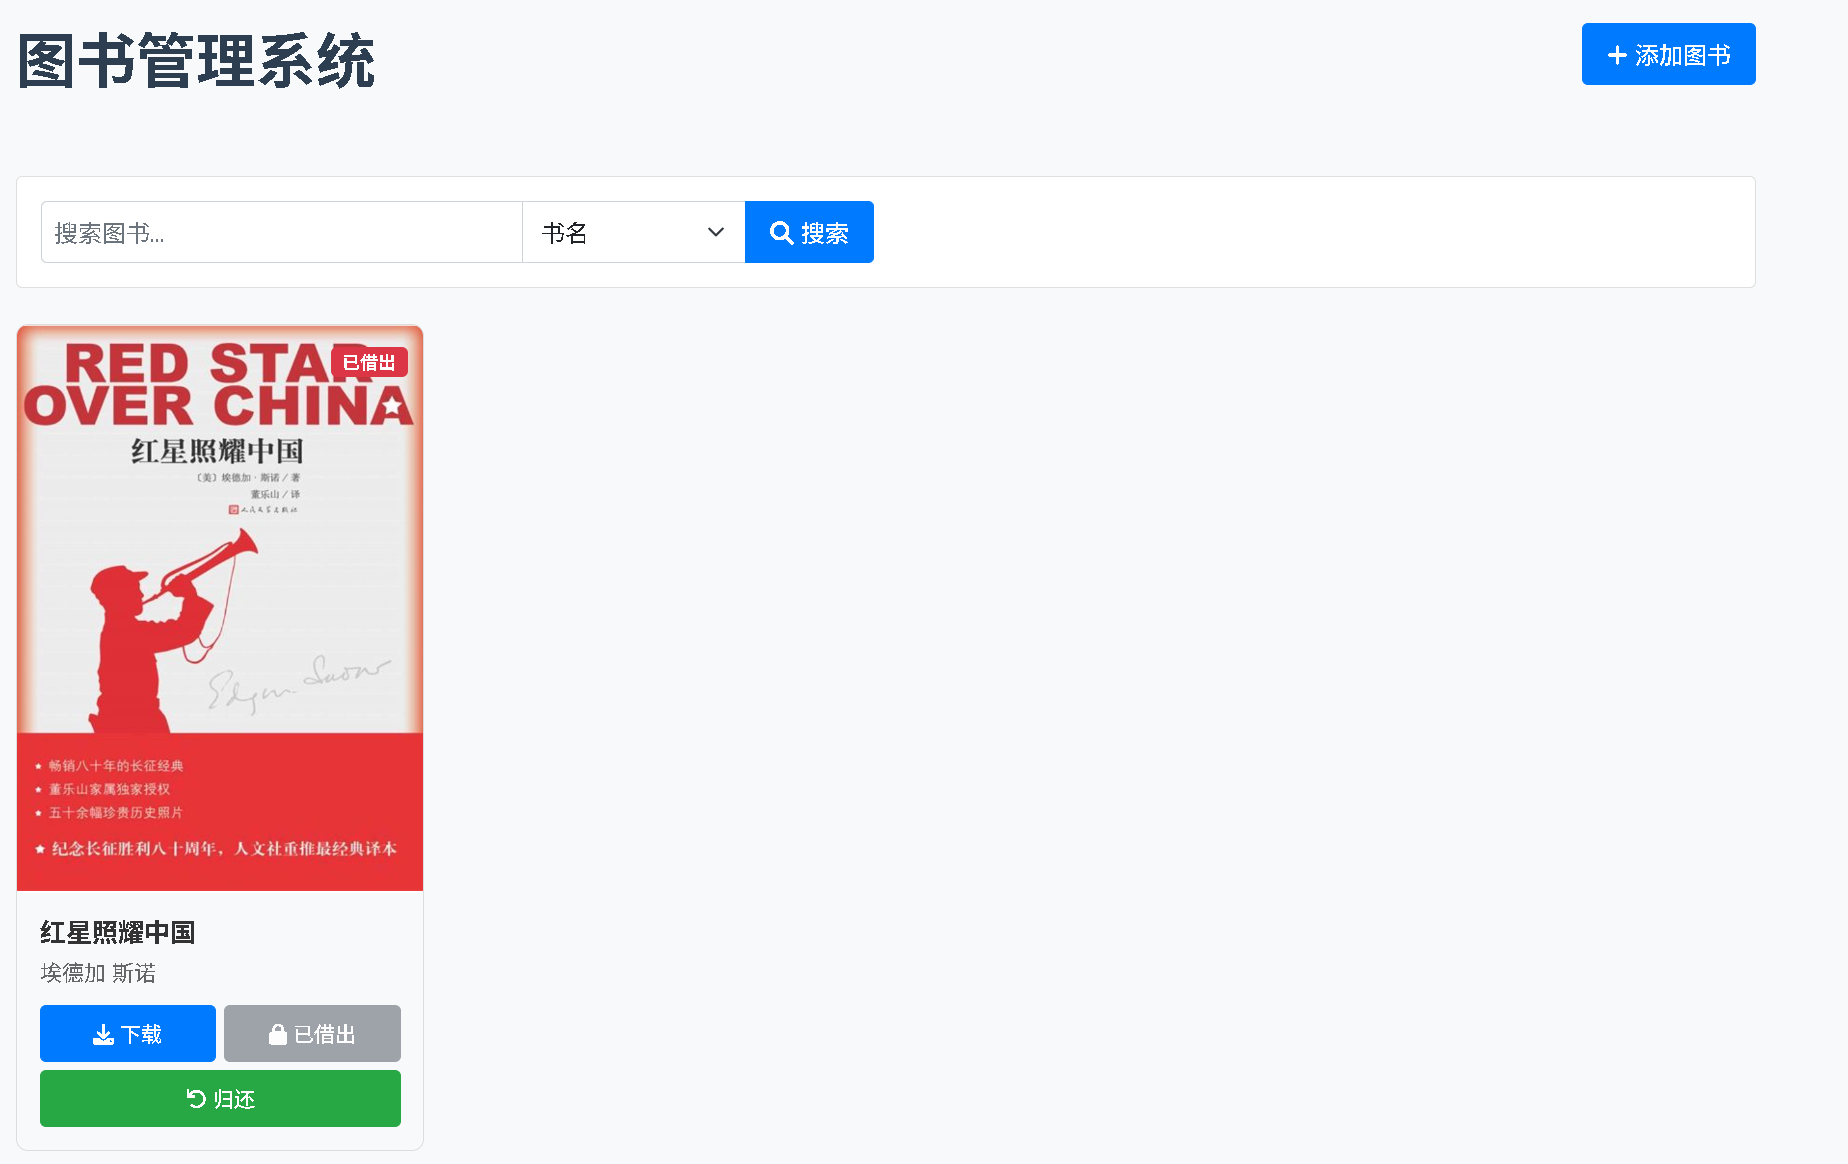
\includegraphics[width=0.9\textwidth]{figures/after_loan.png}
    \caption{借阅图书}
    \label{fig:flow}
\end{figure}

在归还图书后,可以单击图书下方的"删除"按钮实现删除图书。

\begin{figure}[H]
    \centering
    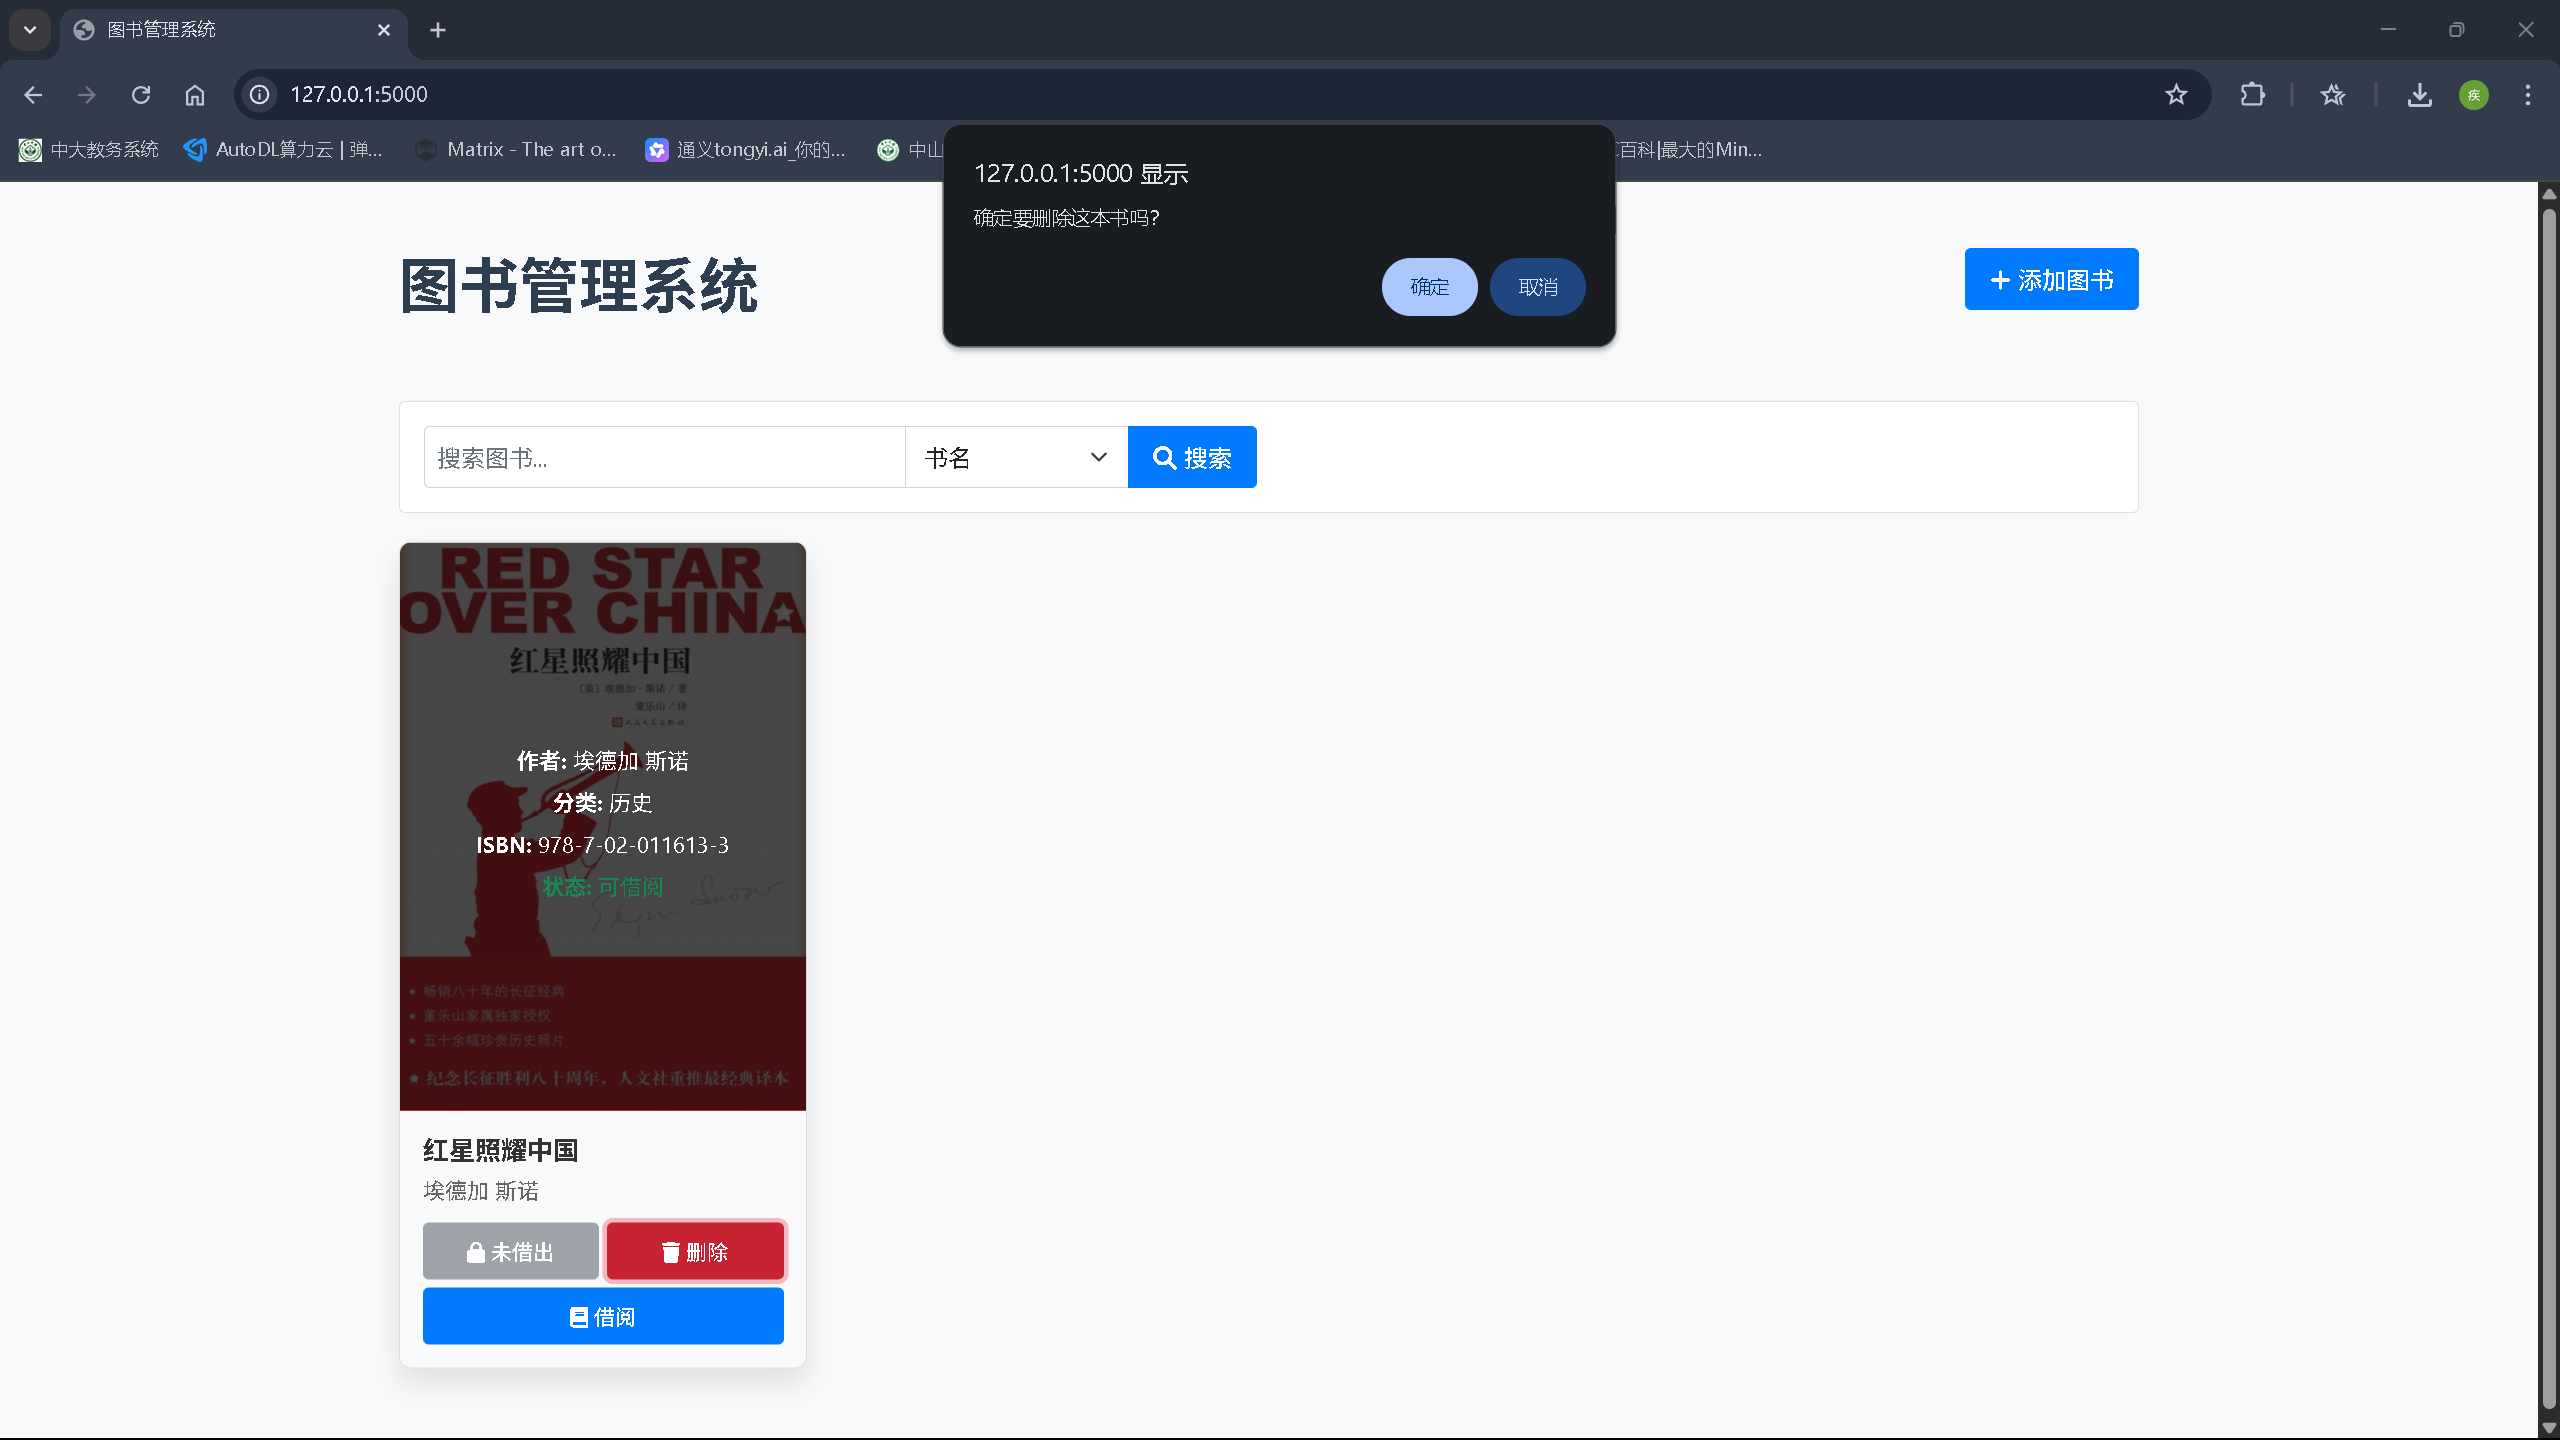
\includegraphics[width=0.9\textwidth]{figures/delete_book.png}
    \caption{删除图书}
    \label{fig:flow}
\end{figure}

\section{总结}

本软件基于ai辅助开发,实现了一个简单的图书管理系统的增、删、查、改功能,体验了人工智能时代软件开发的便利性,为后续开发更加复杂的软件和学习打下了基础。
\end{document}